\documentclass[aspectratio=169, table]{beamer}

%\usepackage[beamertheme=./praditatheme]{Pradita}
\usepackage[utf8]{inputenc}

\usetheme{Pradita}

\subtitle{MTI102-Information Systems \&\\Technology Architecture}

\title{\huge Introduction to\\Enterprise Architecture}
\date[Serial]{\scriptsize {PRU/SPMI/FR-BM-18/0222}}
\author[Pradita]{\small {\textbf{Alfa Yohannis}}}

\begin{document}

    \frame{\titlepage}

    \begin{frame}
        \frametitle{Definition of 'Enterprise' According to }
        \framesubtitle{the Oxford English Dictionary}
        \begin{itemize}
            \item A project or undertaking, usually one that requires effort and courage.
            \item Initiative, dare to take risks to gain profits.
            \item Organization or business company.
        \end{itemize}
    \end{frame}

    \begin{frame}
        \frametitle{Definition of 'Enterprise' According to}
        \framesubtitle{the Cambridge English Dictionary}
        \begin{itemize}
            \item Ability to think about new plans and make them work.
            \item A company.
        \end{itemize}
    \end{frame}

    \begin{frame}
        \frametitle{Definition of 'Enterprise' According to}
        \framesubtitle{Merriam-Webster Dictionary}
        \begin{itemize}
            \item A project or endeavour that often requires courage.
            \item Readiness to engage in bold and risky ventures.
            \item An organized economic unit.
        \end{itemize}
    \end{frame}

    \begin{frame}
        \frametitle{Conclusion to the Definition}
        \framesubtitle{of `Enterprise'}
        \begin{itemize}
            \item 'Enterprise' refers to a bold, risky project or venture.
            \item Can also refer to an organization or business company.
            \item This definition is generally consistent among leading English dictionaries.
        \end{itemize}
    \end{frame}

    \begin{frame}
        \frametitle{Definition of 'Architecture' According to}
        \framesubtitle{the Oxford English Dictionary}
        \begin{itemize}
            \item The art or practice of designing and constructing buildings.
            \item Style or method of construction.
            \item The arrangement or structure of something.
        \end{itemize}
    \end{frame}

    \begin{frame}
        \frametitle{Definition of 'Architecture' According to}
        \framesubtitle{the Cambridge English Dictionary}
        \begin{itemize}
            \item The art and practice of designing buildings.
            \item The style or design of a specific building or group of buildings.
            \item The way something is done or arranged.
        \end{itemize}
    \end{frame}

    \begin{frame}
        \frametitle{Definition of 'Architecture' According to}
        \framesubtitle{Merriam-Webster Dictionary}
        \begin{itemize}
            \item The art or science of designing and constructing buildings.
            \item Method or style of construction.
            \item How the parts of something are arranged or systematized.
        \end{itemize}
    \end{frame}

    \begin{frame}
        \frametitle{Summary}
        \begin{itemize}
            \item 'Architecture' generally refers to the art or practice of designing and constructing buildings.
            \item Can also refer to a style or method of construction.
            \item Additionally, it can also refer to the way the parts of something are arranged or systematized.
        \end{itemize}
    \end{frame}

    \begin{frame}
        \frametitle{Definition of Architecture}
        \framesubtitle{according to IEEE}
        \begin{itemize}
            \item The fundamental organization of a system
            \item Involves system components, relationships between components
            \item Manages system design and evolution
            \item System components can include hardware, software, data, people, processes
        \end{itemize}
    \end{frame}



    \begin{frame}
        \frametitle{Definition of 'Enterprise Architecture'}
        \framesubtitle{According to Gartner}
        \begin{itemize}
            \item A discipline for project design, planning, implementation, and control.
            \item Helps organizations achieve business and IT consistency.
            \item Involves collaboration between various stakeholders.
            \item Can be used to assist in strategic decision-making.
        \end{itemize}
    \end{frame}

    \begin{frame}
        \frametitle{Definition of 'Enterprise Architecture'}
        \framesubtitle{According to TOGAF}
        \begin{itemize}
            \item An architectural framework.
            \item Provides a basic definition and design for enterprise architecture.
            \item Help ensure company operations run consistently and efficiently.
            \item Focuses on standards and procedures used within the company.
        \end{itemize}
    \end{frame}

    \begin{frame}
        \frametitle{Definition of 'Enterprise Architecture'}
        \framesubtitle{According to ISO/IEC/IEEE 42010}
        \begin{itemize}
            \item A fundamental approach to the organization of a system.
            \item Involves understanding all components, the relationships between components, and their environment.
            \item Emphasizes the importance of structure and interactions in systems.
            \item Provides a framework for systems understanding and design.
        \end{itemize}
    \end{frame}



    \begin{frame}
        \frametitle{Various Enterprise Architecture Frameworks}
        \framesubtitle{\hspace{1cm}}
        \begin{itemize}
            \item Business System Planning (BSP)
            \item PRISM Architecture Framework
            \item NIST Enterprise Architecture Model
            \item Zachman Framework
            \item EAP: Enterprise Architecture Planning
            \item Sherwood Applied Business Security Architecture
            \item Federal Enterprise Architecture Framework

        \end{itemize}

    \end{frame}
    \begin{frame}
        \frametitle{Various Enterprise Architecture Frameworks (2)}
        \framesubtitle{\hspace{1cm}}
        \begin{itemize}
            \item Gartner's Enterprise Architecture Method
            \item Department of Defense Architecture Framework (DoDAF)
            \item Australian Government AGA
            \item Business Architecture Body of Knowledge (BizBoK)
            \item ISO Standard for Enterprise Modeling (ISO19439)
        \end{itemize}
    \end{frame}

    \begin{frame}
        \frametitle{Business System Planning}
        \begin{itemize}
            \item This process involves understanding business goals, analyzing business processes, and designing an information system architecture that supports these processes.
            \item BSP helps organizations improve efficiency, simplify operations, and optimize resource allocation.
        \end{itemize}
    \end{frame}

    {
        \setbeamertemplate{navigation symbols}{}
        \setbeamertemplate{footline}{}
        \begin{frame}
            \frametitle{Business System Planning (BSP)}
            \begin{center}
                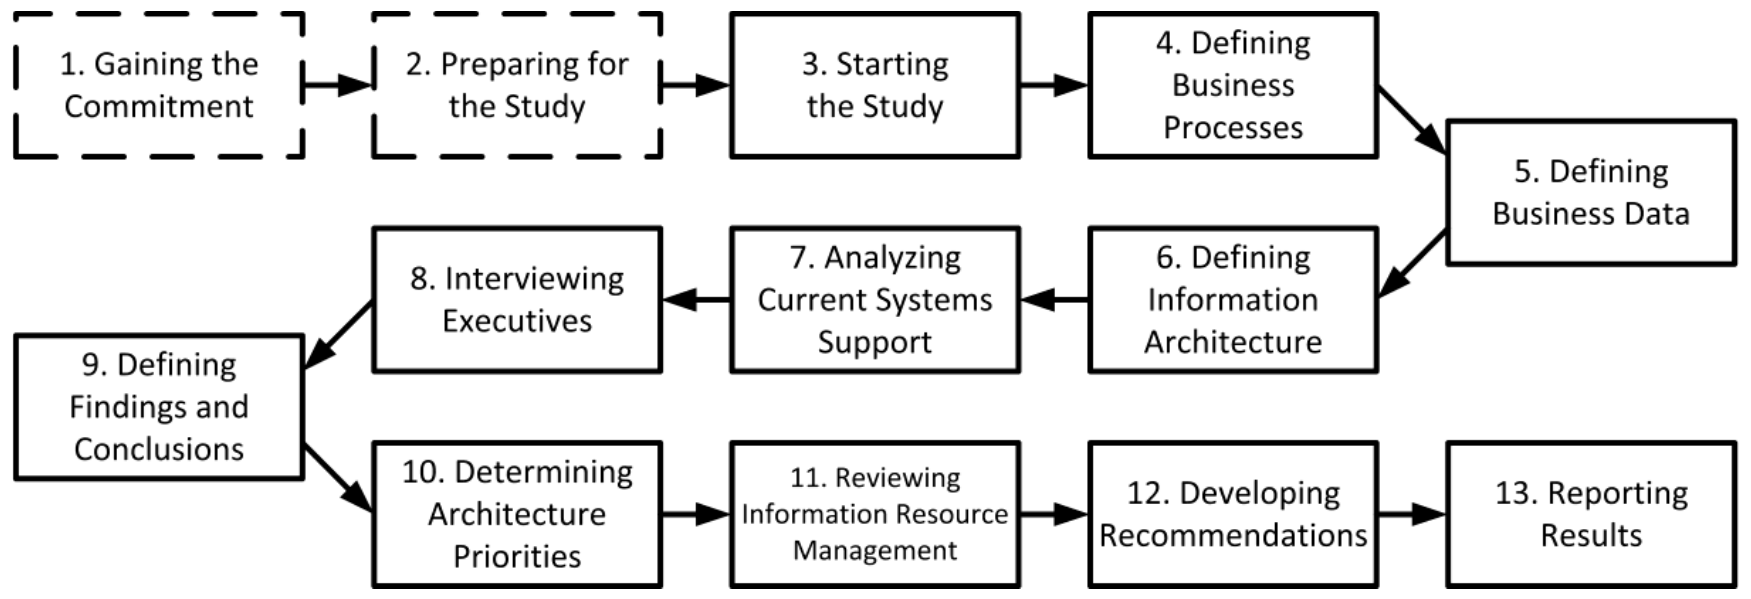
\includegraphics[width=\textwidth]{../figures/bsp}
            \end{center}
        \end{frame}
    }

    \begin{frame}
        \frametitle{PRISM Architecture Framework}
%        \framesubtitle{\hspace{1cm}}
        \begin{itemize}
            \item \textbf{Partnership for Research in Information Systems Management}
            \item One of the first enterprise architecture frameworks
            \item Developed by a consortium of IT vendors
            \item Focuses on system integration and information technology
            \item Helps organizations understand and manage IT complexity
        \end{itemize}
    \end{frame}

    {
        \setbeamertemplate{navigation symbols}{}
        \setbeamertemplate{footline}{}
        \begin{frame}
            \frametitle{PRISM Architecture Framework}
%            \framesubtitle{\hspace{1cm}}
            \begin{center}

                \begin{figure}[ht]
                    \begin{minipage}[b]{0.49\linewidth}
                        \centering
                        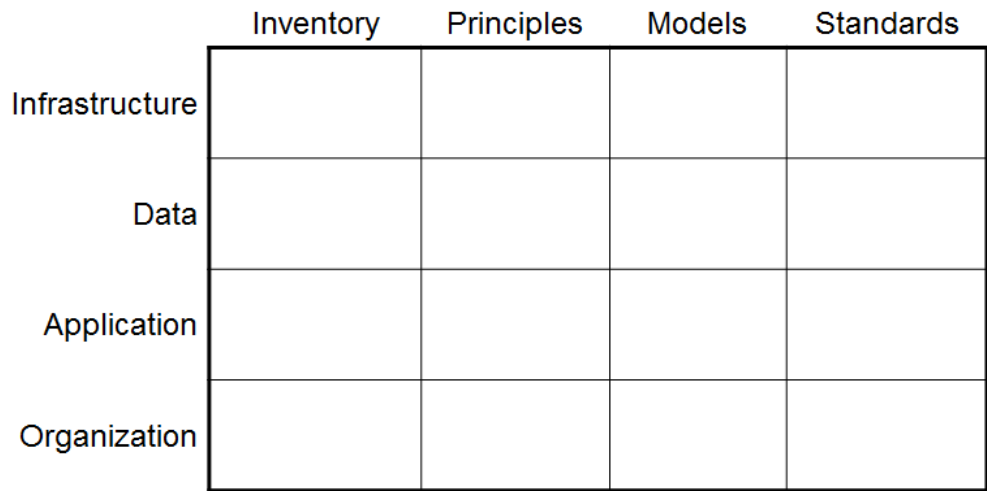
\includegraphics[width=\textwidth]{../figures/prism_matrix}
                        \caption{matrix}
                    \end{minipage}
                    \hfill
                    \begin{minipage}[b]{0.49\linewidth}
                        \centering
                        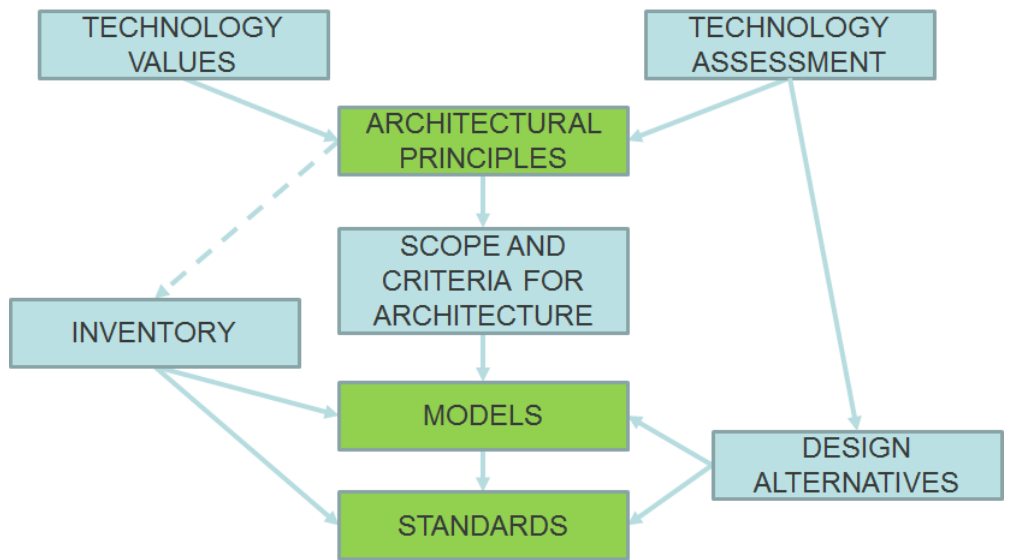
\includegraphics[width=\textwidth]{../figures/prism_relationships}
                        \caption{relationships}
                    \end{minipage}
                \end{figure}

            \end{center}
        \end{frame}
    }

    \begin{frame}
        \frametitle{NIST Enterprise Architecture Model}
        \framesubtitle{\hspace{1cm}}
        \begin{itemize}
            \item  \textbf{National Institute of Standards and Technology}
            \item Emphasizes structuring and organizing IT operations
            \item Divides IT architecture into five levels
            \item Focuses on business, data, applications, technology and results
            \item Enables strategic planning and data-driven decision-making
        \end{itemize}
    \end{frame}

    {
        \setbeamertemplate{navigation symbols}{}
        \setbeamertemplate{footline}{}
        \begin{frame}
            \frametitle{NIST Enterprise Architecture Framework}
            \framesubtitle{\hspace{1cm}}
            \begin{center}
                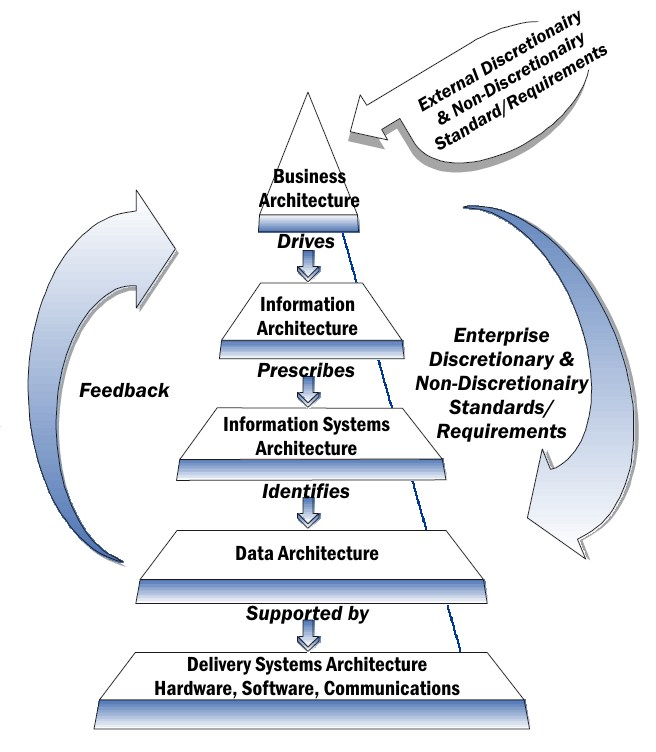
\includegraphics[width=.40\textwidth]{../figures/nist}
            \end{center}
        \end{frame}
    }

    \begin{frame}
        \frametitle{Zachman Framework}
        \begin{itemize}
            \item A schema for understanding and managing the complexity of enterprise architecture
            \item Divided into six different levels
            \item Summarize from the most abstract to the most concrete level
            \item Suitable for many types of organizations, from business to government
        \end{itemize}
    \end{frame}

    {
        \setbeamertemplate{navigation symbols}{}
        \setbeamertemplate{footline}{}
        \begin{frame}
            \frametitle{Zachman Framework}
             \framesubtitle{\hspace{1cm}}
            \vspace{10pt}
            \begin{center}
                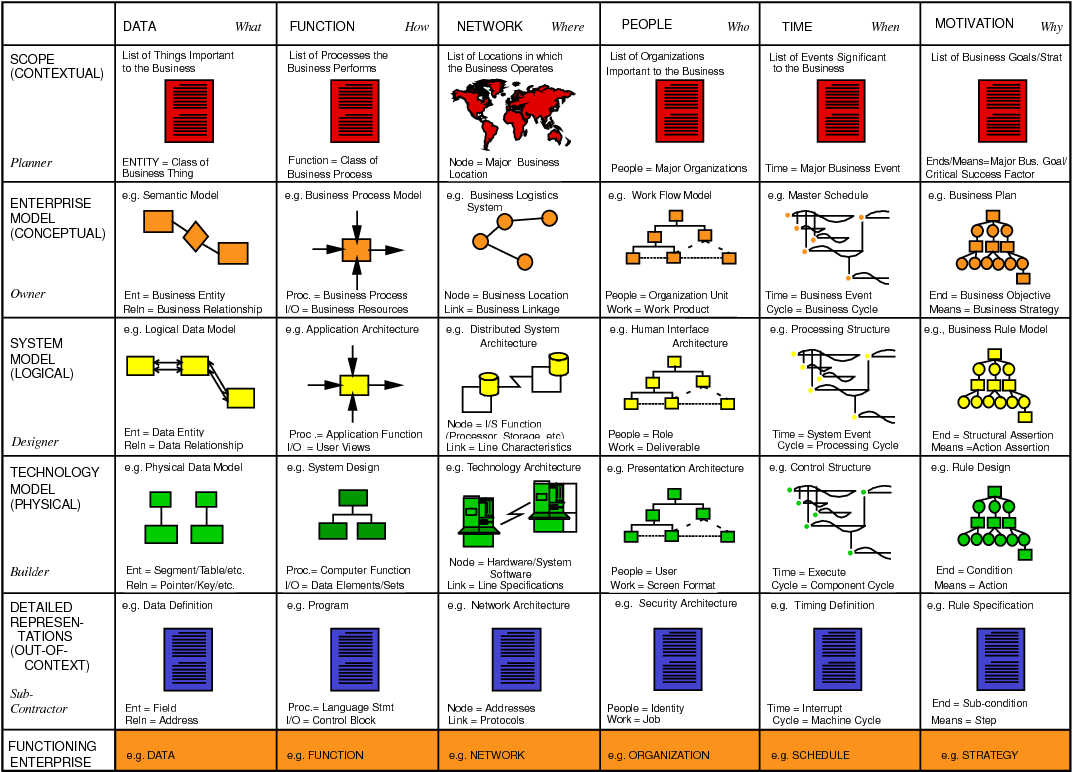
\includegraphics[width=0.76\textwidth]{../figures/zachman}
            \end{center}
        \end{frame}
    }

    \begin{frame}
        \frametitle{Enterprise Architecture Planning (EAP)}
        \framesubtitle{\hspace{1cm}}
        \begin{itemize}
            \item Methods for planning information systems architecture
            \item Identify what the business needs from information technology
            \item Develop plans for implementation of new technology based on business needs
            \item Can help in digital transformation and organizational change
        \end{itemize}
    \end{frame}

    {
        \setbeamertemplate{navigation symbols}{}
        \setbeamertemplate{footline}{}
        \begin{frame}
            \frametitle{Enterprise Architecture Planning}
            \begin{center}
                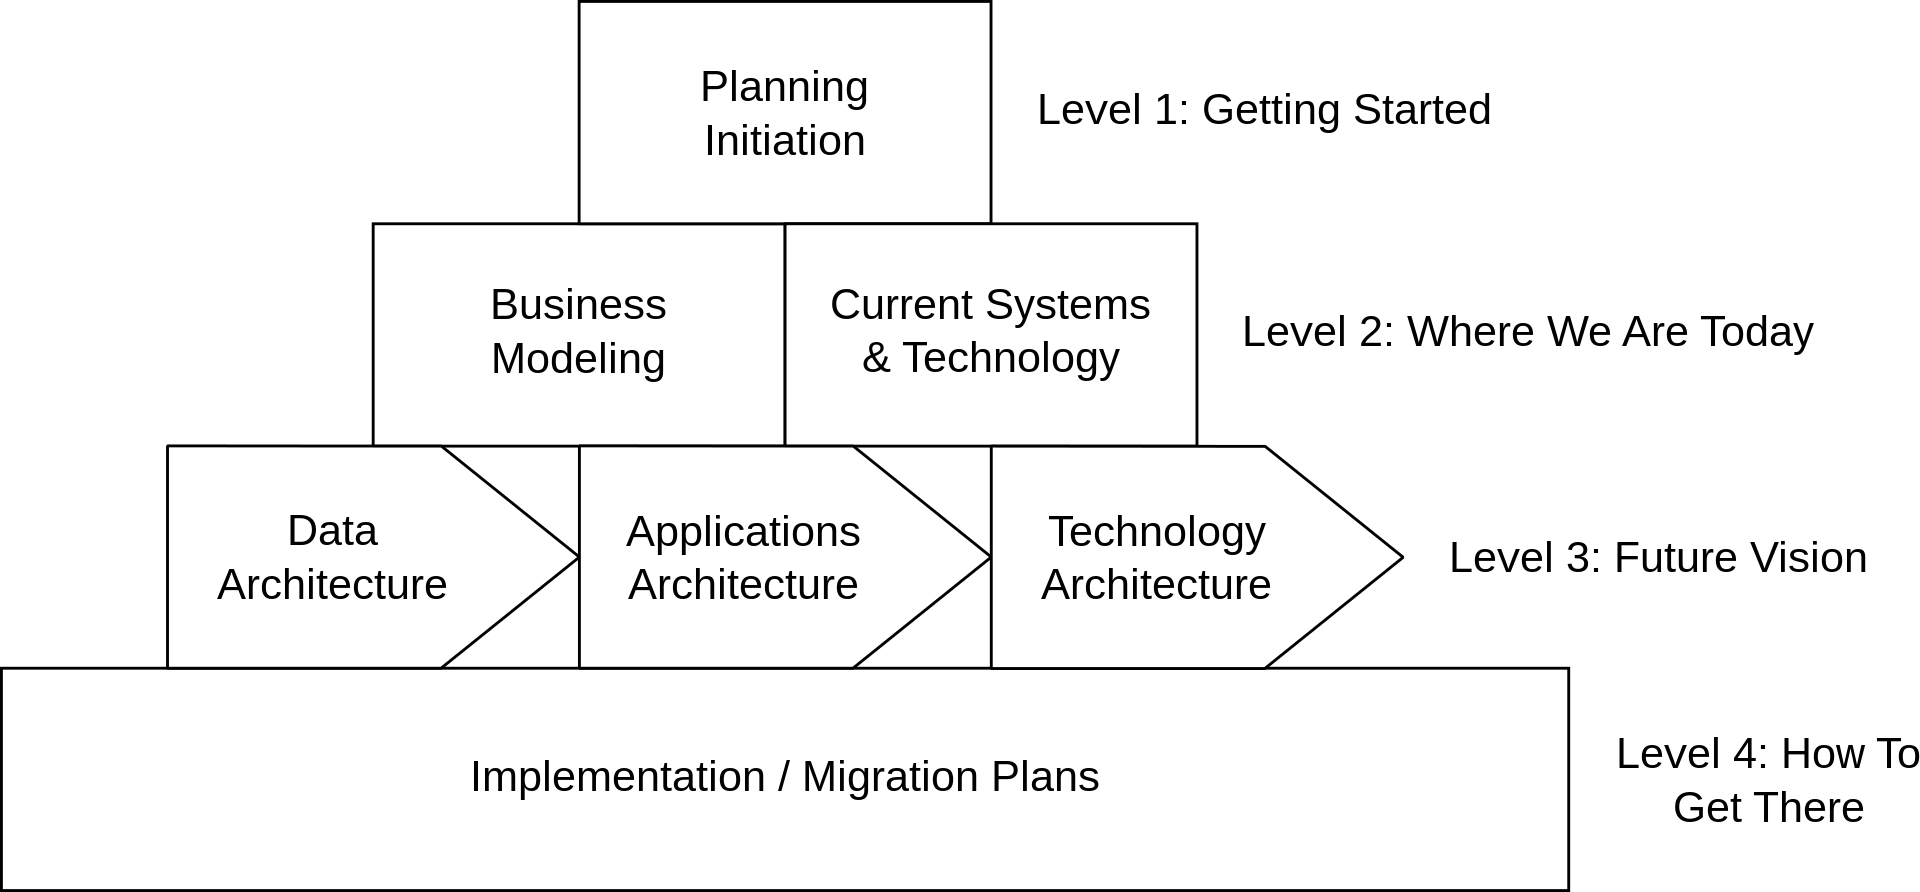
\includegraphics[width=1\textwidth]{../figures/eap}
            \end{center}
        \end{frame}
    }

    \begin{frame}
        \frametitle{Sherwood Applied Business Security Architecture (SABSA)}
        \framesubtitle{\hspace{1cm}}
        \begin{itemize}
            \item Models and methodologies for developing information security and risk management frameworks
            \item Design, implement, and manage business-centric security solutions
            \item Developed with a "start-to-finish" and "top-down" approach
            \item Can be tailored to the specific needs of the organization
        \end{itemize}
    \end{frame}

    {
        \setbeamertemplate{navigation symbols}{}
        \setbeamertemplate{footline}{}
        \begin{frame}
            \frametitle{Sherwood Applied Business Security Architecture (SABSA)}
            \framesubtitle{\hspace{1cm}}
            \begin{center}
                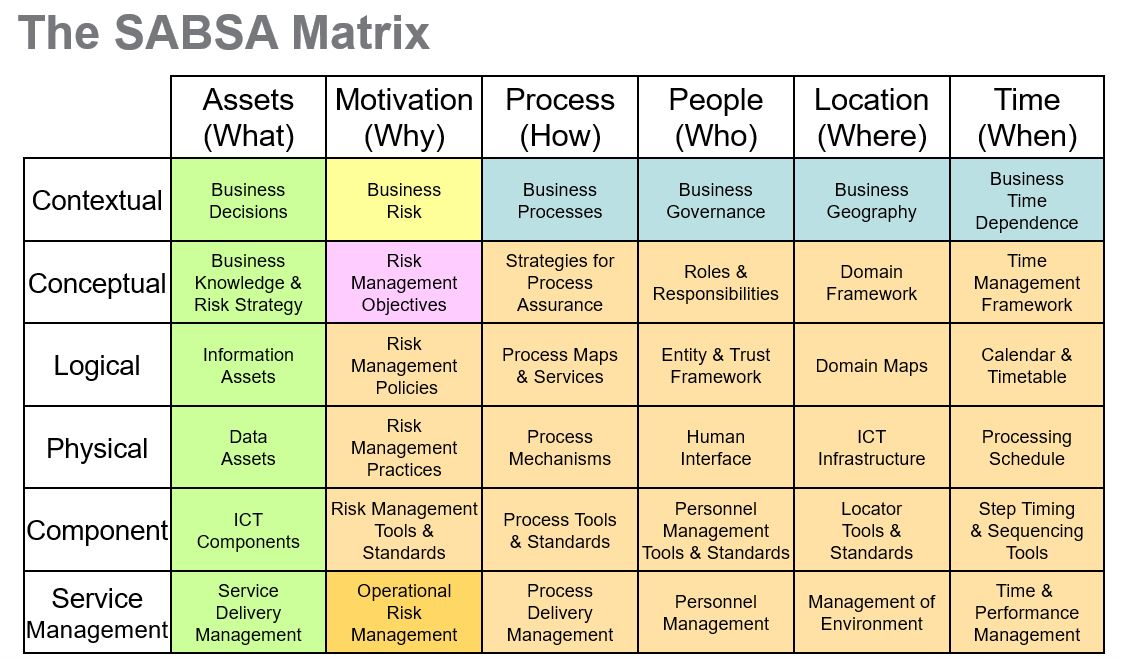
\includegraphics[width=0.8\textwidth]{../figures/sabsa}
            \end{center}
        \end{frame}
    }


    \begin{frame}
        \frametitle{Federal Enterprise Architecture Framework (FEAF)}
        \framesubtitle{\hspace{1cm}}
        \begin{itemize}
            \item Framework used by the US federal government
            \item Helps in improving the efficiency and effectiveness of government services
            \item Facilitate collaboration between government agencies and departments
            \item Is part of the US government's information technology modernization strategy
        \end{itemize}
    \end{frame}

    {
        \setbeamertemplate{navigation symbols}{}
        \setbeamertemplate{footline}{}
        \begin{frame}
            \frametitle{Federal Enterprise Architecture Framework}
            \framesubtitle{\hspace{1cm}}
            \begin{center}
                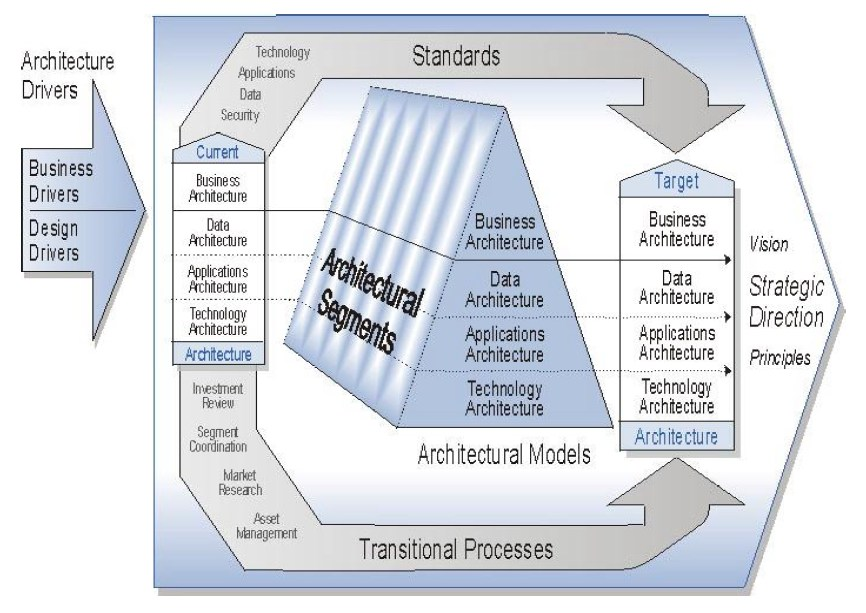
\includegraphics[width=.75\textwidth]{../figures/feaf}
            \end{center}
        \end{frame}
    }

    \begin{frame}
        \frametitle{Gartner Enterprise Architecture Method}
        \framesubtitle{\hspace{1cm}}
        \begin{itemize}
            \item Method developed by the research and consulting company Gartner
            \item Guide organizations in designing, developing, and implementing enterprise architecture
            \item Linking business strategy and IT
            \item Help organizations achieve digital transformation goals
        \end{itemize}
    \end{frame}

    {
        \setbeamertemplate{navigation symbols}{}
        \setbeamertemplate{footline}{}
        \begin{frame}
            \frametitle{Gartner's Enterprise Architecture Process}
            \framesubtitle{\hspace{1cm}}
            \begin{center}
                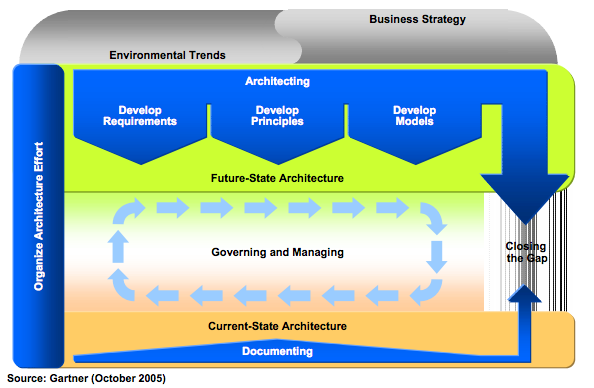
\includegraphics[width=.70\textwidth]{../figures/gartner}
            \end{center}
        \end{frame}
    }

    \begin{frame}
        \frametitle{Department of Defense Architectural Framework (DoDAF)}
        \framesubtitle{\hspace{1cm}}
        \begin{itemize}
            \item Framework used by the US Department of Defense
            \item Helps in organizing and visualizing information important to the decision-making process
            \item Uses various models and guides to develop architecture
            \item Suitable for organizations of large complexity and scale
        \end{itemize}
    \end{frame}

    {
        \setbeamertemplate{navigation symbols}{}
        \setbeamertemplate{footline}{}
        \begin{frame}
            \frametitle{Department of Defense Architecture Framework (DoDAF)}
            \framesubtitle{\hspace{1cm}}
            \begin{center}
                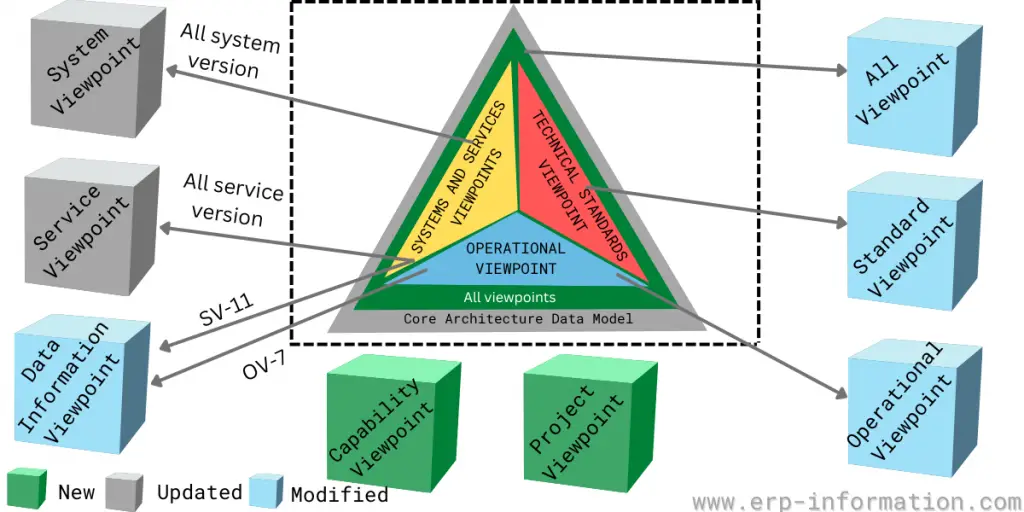
\includegraphics[width=0.68\textwidth]{../figures/dodaf}
            \end{center}
        \end{frame}
    }

    \begin{frame}
        \frametitle{Australian Government AGA}
        \begin{itemize}
            \item Framework used by the Australian Government
            \item Assist in the planning and implementation of information technology at the government level
            \item Encourage collaboration between government departments and agencies
            \item Increase efficiency and transparency in government services
        \end{itemize}
    \end{frame}

    {
        \setbeamertemplate{navigation symbols}{}
        \setbeamertemplate{footline}{}
        \begin{frame}
            \frametitle{Austarlian Government Architecture (AGA)}
            \framesubtitle{\hspace{1cm}}
            \begin{center}
                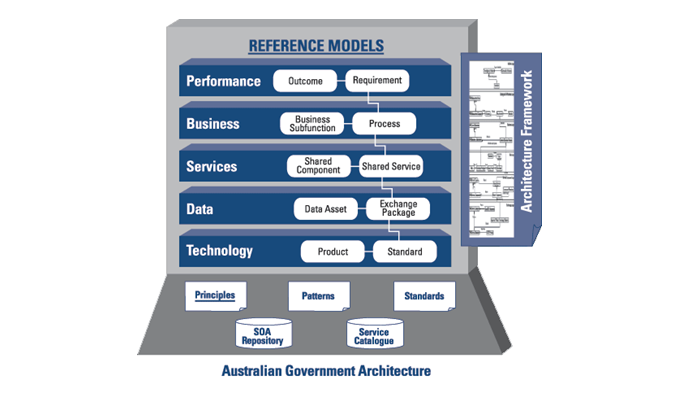
\includegraphics[width=0.9\textwidth]{../figures/aga}
            \end{center}
        \end{frame}
    }

    \begin{frame}
        \frametitle{Business Architecture Body of Knowledge (BizBoK)}
        \framesubtitle{\hspace{1cm}}
        \begin{itemize}
            \item Guide developed by the Business Architecture Guild
            \item Provides best practices and standards in business architecture
            \item Can be used by business architects and other related professionals
            \item Helps organizations in designing and implementing business architecture
        \end{itemize}
    \end{frame}

    {
        \setbeamertemplate{navigation symbols}{}
        \setbeamertemplate{footline}{}
        \begin{frame}
            \frametitle{Business Architecture Body Of Knowledge}
            \framesubtitle{\hspace{1cm}}
            \begin{center}
                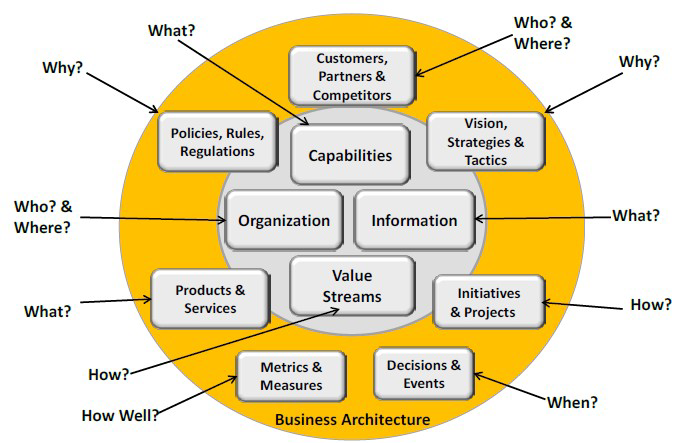
\includegraphics[width=0.7\textwidth]{../figures/bizbok}
            \end{center}
        \end{frame}
    }

    \begin{frame}
        \frametitle{ISO Standard for Enterprise Modeling (ISO19439)}
        \framesubtitle{\hspace{1cm}}
        \begin{itemize}
            \item International standard for modelling business and organizational processes
            \item Assists in planning, design, and improvement of business processes
            \item Can be used by many types of organizations, from business to government
            \item Developed by the International Organization for Standardization (ISO)
        \end{itemize}
    \end{frame}

    {
        \setbeamertemplate{navigation symbols}{}
        \setbeamertemplate{footline}{}
        \begin{frame}
            \frametitle{ISO19439 Enterprise Modelling}
            \begin{center}
                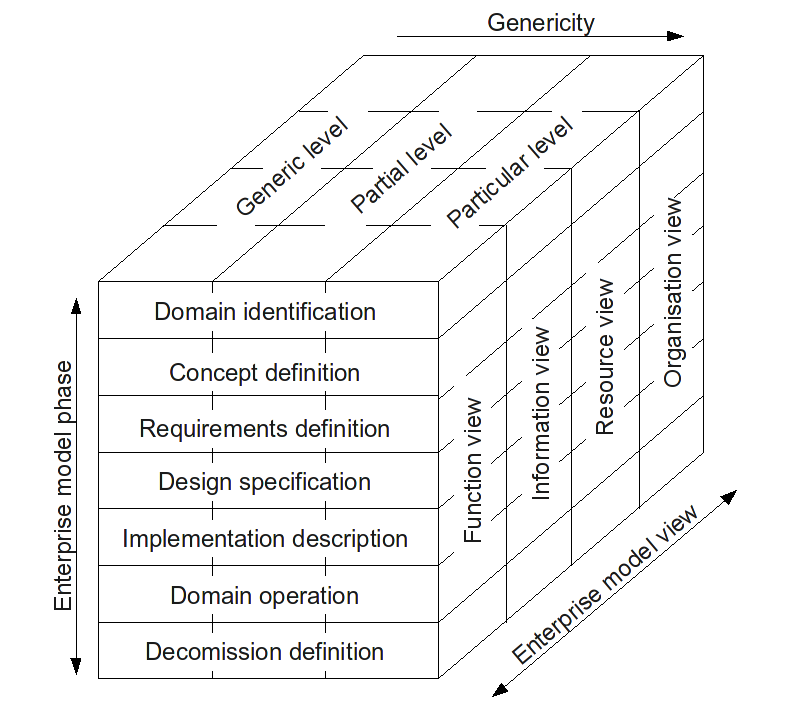
\includegraphics[width=.45\textwidth]{../figures/iso19439}
            \end{center}
        \end{frame}
    }

    \begin{frame}
        \frametitle{Summary}
        \begin{itemize}
            \item There are various enterprise architecture frameworks and methodologies
            \item The choice of framework or methodology depends on the organization's specific needs and context
            \item Enterprise architecture is an important tool for planning and managing information technology in organizations
        \end{itemize}
    \end{frame}



\section{Example of Organization's Vision and Mission}

\begin{frame}
	\centering
	\Huge Example of Organization's Vision and Mission
\end{frame}

\begin{frame}{Vision}
	To become a globally recognized higher education institution, driving innovation, integrity, and inclusivity, while shaping leaders who contribute to a sustainable and just world.
\end{frame}

\begin{frame}{Mission}
	\begin{enumerate}
		\item \textbf{Deliver High-Quality Education:} Provide transformational education that prepares students to excel in their chosen fields through cutting-edge curricula, critical thinking, and practical experience.
		\item \textbf{Promote Research and Innovation:} Foster a culture of research, creativity, and innovation to address societal challenges and advance knowledge across disciplines.
		\item \textbf{Develop Ethical and Environmental Leadership:} Cultivate leaders with strong ethical values, social responsibility, and environmental consciousness, promoting sustainable practices and a commitment to positive change in both local and global communities.
		\item \textbf{Encourage Inclusivity and Diversity:} Create a diverse and inclusive learning environment that values and embraces differences, ensuring equal opportunities for all members of the university community.
		\item \textbf{Collaborate with the Community:} Build partnerships with industry, government, and civil society to address societal needs and contribute to national and global development.
	\end{enumerate}
\end{frame}

\section{SWOT Analysis Example}

\begin{frame}
	\centering
	\Huge SWOT Analysis Example
\end{frame}

\begin{frame}{Strengths}
	\begin{itemize}
		\item \textbf{Global Reputation:} The university is globally recognized for its high-quality academic programs and focus on innovation.
		\item \textbf{Outstanding Research Facilities:} Equipped with state-of-the-art laboratories and research centers that support innovation and research across multiple disciplines.
		\item \textbf{Ethical and Environmental Leadership:} Committed to developing leaders who are not only ethical but also environmentally conscious and committed to sustainability.
		\item \textbf{Diversity and Inclusivity:} The university offers an inclusive environment that values diversity within its academic community.
	\end{itemize}
\end{frame}

\begin{frame}{Weaknesses}
	\begin{itemize}
		\item \textbf{Limited Research Funding:} Despite having excellent facilities, the university faces limited funding for research in certain fields.
		\item \textbf{Lack of International Collaboration:} The university has room to strengthen partnerships with foreign universities to improve exchange programs and collaborative research.
		\item \textbf{Underdeveloped Online Programs:} Development of distance education and online learning programs is still in its early stages and not yet fully optimized.
	\end{itemize}
\end{frame}

\begin{frame}{Opportunities}
	\begin{itemize}
		\item \textbf{Growing Demand for Sustainability Education:} With increasing global attention to environmental issues, there is an opportunity to expand programs focused on sustainability and green innovation.
		\item \textbf{Collaboration with Industry:} The university can expand partnerships with the industrial sector to enhance curriculum relevance and increase internship and applied research opportunities.
		\item \textbf{Advances in Digitalization:} Technological advancements enable the university to expand its reach by developing more online and hybrid learning programs.
	\end{itemize}
\end{frame}

\begin{frame}{Threats}
	\begin{itemize}
		\item \textbf{Global Competition:} The university faces strong competition from global institutions offering high-quality programs focused on innovation.
		\item \textbf{Changing Education Regulations:} Changes in government policies or regulations related to higher education could impact the sustainability of programs and university operations.
		\item \textbf{Shifts in Education Trends:} A shift in student preferences towards fully online learning could reduce interest in traditional education programs.
	\end{itemize}
\end{frame}

\section{Porter's Five Forces Model Analysis}

\begin{frame}
	\centering
	\Huge Porter's Five Forces Model Analysis
\end{frame}

\begin{frame}{Threat of New Entrants}
	\begin{itemize}
		\item \textbf{New Competition:} The rise of new universities focusing on technology and online learning could increase competition in the higher education sector.
		\item \textbf{High Barriers to Entry:} Universities with a global reputation and outstanding research facilities face lower threats from new entrants, as it requires significant investment to match their infrastructure and reputation.
		\item \textbf{Technological Innovation:} New universities offering cutting-edge technology-based education programs may provide attractive alternatives for prospective students.
	\end{itemize}
\end{frame}

\begin{frame}{Supplier Power (Faculty and Experts)}
	\begin{itemize}
		\item \textbf{Availability of Experts:} Universities require high-quality faculty with specialized expertise. The competition to attract top professors poses a challenge for the university.
		\item \textbf{Dependence on Key Figures:} High dependence on prominent professors or experts in certain fields can be risky if they leave the institution or retire.
		\item \textbf{Research and Innovation Facilities:} Excellent research facilities give the university a greater advantage in attracting and retaining top faculty members.
	\end{itemize}
\end{frame}

\begin{frame}{Buyer Power (Students and Parents)}
	\begin{itemize}
		\item \textbf{Wider Choices:} Prospective students have many options, including other universities and online learning programs, which may be more flexible and affordable.
		\item \textbf{Student Demands:} Students increasingly demand higher education quality, modern facilities, and strong career opportunities, requiring universities to continuously innovate in curriculum and services.
		\item \textbf{Parental Role:} Parents also play a crucial role in university selection, particularly regarding tuition costs and the future prospects of graduates.
	\end{itemize}
\end{frame}

\begin{frame}{Threat of Substitute Products or Services}
	\begin{itemize}
		\item \textbf{Online Learning:} Fully online programs from major universities or education platforms like Coursera and edX could pose a significant threat to universities that still focus on traditional learning.
		\item \textbf{Professional Certification Courses:} Professional certifications offered by tech companies or training institutions can serve as alternatives for students seeking shorter, more focused learning instead of traditional university education.
		\item \textbf{Internship or Work Training Programs:} The rising popularity of direct internship or work training programs offered by companies could also serve as an alternative for students seeking practical experience.
	\end{itemize}
\end{frame}

\begin{frame}{Rivalry Among Competitors}
	\begin{itemize}
		\item \textbf{Global Competition:} Universities face competition from global education institutions offering similar programs at international standards, either directly or through online platforms.
		\item \textbf{Curriculum Innovation:} Other universities that are quicker to adopt innovative curricula or more flexible learning approaches may attract more students.
		\item \textbf{Reputation and Alumni Network:} The strength of an institution's alumni network and reputation is critical in attracting new students and maintaining a competitive edge.
	\end{itemize}
\end{frame}

\section{PEST Analysis}

\begin{frame}
	\centering
	\Huge PEST Analysis
\end{frame}

\begin{frame}{Political Factors}
	\begin{itemize}
		\item \textbf{Government Education Policies:} Changes in government policies can directly impact the curriculum, accreditation, and financial support provided to universities.
		\item \textbf{Political Stability:} A stable political environment allows universities to focus on long-term strategies and partnerships, while instability can disrupt operations and planning.
		\item \textbf{Regulations on Research:} Regulations on research funding and intellectual property rights affect the university's ability to innovate and collaborate with industry partners.
	\end{itemize}
\end{frame}

\begin{frame}{Economic Factors}
	\begin{itemize}
		\item \textbf{Economic Growth:} Strong economic growth increases the demand for higher education as more individuals seek advanced qualifications to remain competitive in the job market.
		\item \textbf{Tuition Fees and Student Debt:} Rising tuition fees and concerns over student debt can impact the ability of students to afford higher education.
		\item \textbf{Funding and Grants:} The availability of public or private funding and research grants influences the university’s ability to invest in research and development.
	\end{itemize}
\end{frame}

\begin{frame}{Social Factors}
	\begin{itemize}
		\item \textbf{Demographic Changes:} Shifts in population demographics, such as aging populations or a growing youth population, can affect enrollment numbers and program offerings.
		\item \textbf{Cultural Attitudes toward Education:} Social and cultural attitudes toward higher education influence student choices, including preferences for certain fields of study and career aspirations.
		\item \textbf{Emphasis on Lifelong Learning:} As industries evolve, there is increasing demand for lifelong learning programs and continuing education, which universities can leverage.
	\end{itemize}
\end{frame}

\begin{frame}{Technological Factors}
	\begin{itemize}
		\item \textbf{E-Learning Platforms:} The rise of e-learning platforms presents both an opportunity and a challenge for traditional universities, requiring them to adapt to digital transformation.
		\item \textbf{Technological Advancements:} Advances in artificial intelligence, data analytics, and digital tools offer new opportunities for enhancing educational experiences and research capabilities.
		\item \textbf{Infrastructure Requirements:} Universities must invest in up-to-date technological infrastructure to support modern learning and research needs effectively.
	\end{itemize}
\end{frame}

\begin{frame}{Legal Factors}
	\begin{itemize}
		\item \textbf{Education Regulations:} Compliance with national and international regulations regarding accreditation, curriculum, and copyright.
		\item \textbf{Intellectual Property Rights:} Protection of copyrights and patents resulting from university research.
		\item \textbf{Employment Regulations:} Compliance with labor laws and policies protecting the rights of faculty and staff.
	\end{itemize}
\end{frame}

\begin{frame}{Environmental Factors}
	\begin{itemize}
		\item \textbf{Environmental Awareness:} Implementation of environmentally friendly policies in campus management, such as reducing carbon footprints and using renewable energy sources.
		\item \textbf{Sustainable Program Development:} Development and offering of programs focused on sustainability and environmental issues.
		\item \textbf{Resource Management:} Practices for efficient management of natural resources to support campus sustainability.
	\end{itemize}
\end{frame}

\begin{frame}
	\centering
	\Huge Innovations and Latest IT Technologies to Enhance University Quality
\end{frame}

\begin{frame}{Online and Hybrid Learning}
	\begin{itemize}
		\item \textbf{Online Learning Platforms:} Use of platforms such as Moodle, Blackboard, or Canvas to provide online courses, learning modules, and student-faculty interactions.
		\item \textbf{Virtual Classrooms:} Implementation of virtual classroom technologies such as Zoom or Microsoft Teams for live lectures and online discussion sessions.
		\item \textbf{Augmented Reality (AR) and Virtual Reality (VR):} Integration of AR and VR to provide immersive learning experiences, such as lab simulations or virtual tours of historical sites.
	\end{itemize}
\end{frame}

\begin{frame}{Data Analysis and Artificial Intelligence}
	\begin{itemize}
		\item \textbf{AI-Based Learning Management Systems:} Use of artificial intelligence to tailor the learning experience to individual student needs and provide automated feedback.
		\item \textbf{Learning Analytics:} Implementation of analytics tools to monitor student progress, identify areas needing attention, and adjust the curriculum based on performance data.
		\item \textbf{Academic Chatbots:} Use of AI-based chatbots to answer student questions about administration, schedules, and course materials in real-time.
	\end{itemize}
\end{frame}

\begin{frame}{IT Security and Infrastructure}
	\begin{itemize}
		\item \textbf{Cybersecurity:} Implementation of advanced cybersecurity systems to protect student and research data from cyber threats, including data encryption and intrusion detection systems.
		\item \textbf{Cloud Computing:} Use of cloud services for data storage, collaboration, and scalability to enhance university operational flexibility and efficiency.
		\item \textbf{Internet of Things (IoT):} Integration of IoT to monitor and manage campus facilities more efficiently, such as automated lighting systems and temperature controls.
	\end{itemize}
\end{frame}

\begin{frame}{Curriculum Development and Innovation}
	\begin{itemize}
		\item \textbf{Online Courses and Certifications:} Offering online courses and certifications relevant to the latest industry trends to broaden students' knowledge beyond traditional curricula.
		\item \textbf{Virtual Laboratories:} Use of virtual labs for experiments and practices that allow students to conduct research without being physically present in a lab.
		\item \textbf{Research Collaboration Platforms:} Use of online platforms for research collaboration between students, faculty, and researchers from other universities or industries.
	\end{itemize}
\end{frame}

\begin{frame}{Enhancing Student Experience}
	\begin{itemize}
		\item \textbf{University Mobile Apps:} Development of mobile apps to facilitate student access to campus information, schedules, course materials, and administrative services.
		\item \textbf{Mental Health Monitoring Systems:} Implementation of tools and apps to monitor and support student mental health, such as online counseling platforms and wellness tracking apps.
		\item \textbf{Virtual Campus Tours:} Provision of virtual campus tours for prospective students and parents to explore facilities and campus atmosphere remotely.
	\end{itemize}
\end{frame}

\begin{frame}
	\centering
	\Huge Interview Results with Students, Staff, and Faculty
\end{frame}

\begin{frame}{Issues Faced by Students}
	\begin{itemize}
		\item \textbf{Parking Difficulties:} Students report difficulties in finding parking on campus, especially during peak hours, leading to delays and stress.
		\item \textbf{Manual Attendance:} Manual attendance processes result in delays in recording attendance and require additional effort for verification.
		\item \textbf{Duplicate Documents:} Students face issues with documents that need to be filled out repeatedly in various places, wasting time and reducing efficiency.
	\end{itemize}
\end{frame}

\begin{frame}{Issues Faced by Staff}
	\begin{itemize}
		\item \textbf{Unclear Business Processes:} Staff report that some business processes at the university are poorly documented or unclear, leading to confusion and uncertainty in task execution.
		\item \textbf{Unclear Responsibilities:} There is ambiguity regarding the division of responsibilities and authority in some departments, causing conflicts and delays in completing tasks.
		\item \textbf{Duplicate Internal Documentation:} Mismanagement of internal documents leads to repetitive copies and potential errors or loss of information.
	\end{itemize}
\end{frame}

\begin{frame}{Issues Faced by Faculty}
	\begin{itemize}
		\item \textbf{Administrative Delays:} Faculty experience delays in administrative processes, such as course registration and grade processing, which disrupt efficiency and teaching schedules.
		\item \textbf{Lack of Teaching Aids:} Faculty report a lack of adequate teaching aids and technology to support the learning and research process.
		\item \textbf{Inefficient Communication:} Problems in communication between faculty and administration or between faculty and students lead to confusion and delays in resolving academic tasks or issues.
	\end{itemize}
\end{frame}


\end{document}